\chapter{Função Logarítmica}
\section{Logaritmos}
\subsection{Breve Histórico}

Na Idade Média o trabalho dos físicos e astrônomos para realizar grandes operações aritméticas era longo, extremamente exaustivo e tedioso. Na ausência de calculadoras e notações convenientes, várias horas eram perdidas com pequenos erros que traziam um grande atraso para toda ciência.
\marginpar{
	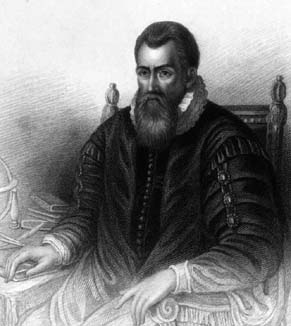
\includegraphics[width=0.85\marginparwidth]{imagens/napier.jpeg}
	\captionof{figure}{John Napier}
	\label{fig:napier}}
	
	
Vários métodos haviam sido inventados para simplificar tais operações, mas o que se tornaria mais famoso, sem dúvidas, seria o invento de John Napier: \margem{John Napier foi um matemático e físico escocês que viveu entre o fim do século XVI e o começo do século XVII. Sua vida de trabalho dedicada, entre outras coisas, a invenção do logaritmo foi um impulso decisivo para Kepler e outros cientistas da época.}o logaritmo.

O logaritmo foi uma invenção importantíssima pois permitiu, com tabelas apropriadas, substituir multiplicações por adições segundo a seguinte propriedade: $$\log{(a.b)} = \log{a} + \log{b}$$

Dessa forma, se quiséssemos saber o resultado do produto $a.b$, consultaríamos o valor de $\log{a}$ e $\log{b}$ em uma tabela, faríamos a soma de $\log{a}$ e $\log{b}$ e depois verificaríamos, em uma outra tabela, qual o número cujo resultado é igual a soma anterior.

Essa propriedade (tida como miraculosa) simplificou e agilizou longos cálculos, disseminando-se rapidamente por toda a Europa. A definição que veremos abaixo de logaritmo se deve ao brilhante matemático Leonhard Euler, que conectou a teoria dos logaritmos com a teoria das exponenciais, tornando a invenção de Napier útil não só para efetuar longas multiplicações mas também fundamental para a matemática pura.

\subsection{Definição}

Nas aulas sobre Função Exponencial vimos que a função exponencial é inversível, desde que sua base seja diferente de 1. Vamos construir a função logaritmo partindo desse princípio. O logaritmo será definido como a função inversa da exponencial. Assim, por exemplo: $$\log_2{8}=3 \text{  pois  } 2^3=8$$ $$\log_9{3} = \frac{1}{2} \text{  pois  } 9^{\frac{1}{2}}=3$$

\label{def:log}\definicao{\textbf{Logaritmo} \\ \begin{center}
Sejam $a$ e $b$ números reais positivos e $b \ne 1$
\newline \newline
$\log_b{a}$ é a (única) raiz da equação $b^x=a$ 
\newline \newline
($x$ é chamado de logaritmo de $a$ na base $b$. $b$ é chamado de base, $a$ é chamado de logaritmando)
\end{center}
}\\

\exem{Titulo}{\begin{enumerate}[a)]
\item $\log_2{\frac{1}{8}}$ é a raiz da equação $2^x=\frac{1}{8}$, assim $2^x=2^{-3}$ e $\log_2{\frac{1}{8}}=-3$ 

\item $\log_{10}{1}$ é a raiz da equação $10^x=1$, assim $\log_{10}{1}=0$

\item $\log_{\frac{1}{4}}{16}$ é a raiz da equação $\frapar{1}{4}^x=16$. Assim $\log_{\frac{1}{4}}{16}=-2$
\end{enumerate}
}

Seguem imediatamente da definição de logaritmo as seguintes propriedades

\margem{O nome logaritmo vem do grego e significa número que representa uma razão. Podemos entender esse nome se pensarmos que $\log_2{2}$, $\log_2{4}$, $\log_2{8}$, $\log_2{16}$,$\ldots$ onde o logaritmando cresce geometricamente, representa $1,2,3,4,\ldots$ sequencia em que os números crescem aritmeticamente.
}
\caixaprop{
\begin{propriedade}\label{prop:log_nuvem}
$\log_b{a}=c \Leftrightarrow b^c=a$
\end{propriedade}
\begin{propriedade}\label{prop:log_inversa}
$\log_b{b^x}=x$
\end{propriedade}
\begin{propriedade}\label{prop:log_inversa2}
$b^{\log_b{x}}=x$
\end{propriedade}
}

\exem{Titulo}{ \begin{enumerate}[a)]

\item $27^{\log_3{5}} = (3^3)^{\log_3{5}} = (3^{\log_3{5}})^3 = 5^3 = 125$
\item $2^{\log_2{3}-1} = \frac{2^{\log_2{3}}}{2^1}=\frac{3}{2}$
\item $\log_9{27} = \log_9{3^3}=\log_9{9^{\frac{3}{2}}} = \frac{3}{2}$


\end{enumerate}
}

Comparando as propriedades básicas de exponenciação chegamos em mais algumas propriedades dos logaritmos:

\caixaprop{Seja $b$ um número real positivo e diferente de 1, então

\begin{propriedade} $\log_b{1}=0$, pois $b^0=1$
\end{propriedade}

\begin{propriedade}\label{prop:logbbaseb} $\log_b{b}=1$, pois $b^1=b$
\end{propriedade}
}

\begin{exeresol}[INTERDISCIPLINAR] Calcule o $pH$ de uma solução de $0.1$ mol de ácido clorídrico em um recipiente de $10 L$.\\
\textbf{Solução}\\
Como o ácido clorídrico é um ácido forte ele sofre ionização praticamente completa. Como $$HCl \to H^+ + Cl^-$$Temos que $0.1$ mol de $HCl$ formam $0.1$ mol de $H^+$. A concentração de $H^+$ então é $M = \frac{n}{V} = \frac{0.1}{10} = 10^{-2} mol/L$ e assim $pH= -\log_{10}{10^{-2}} = - (-2) = 2$ e o $pH$ da solução é $2$.
\end{exeresol}
\margem{O $pH$ de uma solução química é dado pela fórmula $pH = -\log_{10}{[H^+]}$, onde $[H^+]$ representa a concentração em $mol/L$ do cátion $H^+$.}
\comecaexer
\subsection*{Exercícios}
Se você estiver com dificuldade ao resolver esses exercícios reveja a última aula sobre função exponencial e faça alguns exercícios sobre equações exponenciais.
\begin{exer}Calcule pela definição
\begin{enumerate}[a)]
\item $\log_2{(\frac{1}{2})}$
\item $\log_4{128}$
\item $\log_{\frac{1}{2}}{(\frac{1}{8})}$
\item $\log_{0.125}{4}$
\item $\log_3{(\frac{1}{9})}$
\item $\log_{25}{5}$
\item $\log_{\sqrt{2}}{16}$
\item $\log_{\sqrt[3]{5}}{125}$
\item $\log_{\pi}{\pi^2}$
\item $\log_{50}{1}$
\item $\log_4{(\log_3{9})}$
\end{enumerate}
\end{exer}

\begin{exer} Seja $f \colon \R \to \Rep^*$ a função exponencial de base $3$. (Ou seja, $f(x)=3^x$). Faça o que se pede:
\begin{enumerate}[a)]
\item Esboce o gráfico de $f$
\item No mesmo sistema cartesiano do item anterior, esboce o gráfico de $f^{-1}$ (Lembrete: O gráfico de uma função e de sua inversa são simétricos em relação a reta $y=x$, bissetriz dos quadrantes ímpares)
\item Calcule $f^{-1}(9)$, $f^{-1}(27)$ e $f^{-1}(\sqrt{3})$
\end{enumerate}
\end{exer}

\begin{exer}[MACKENZIE] A expressão $\log_{\frac{1}{2}}32 + \log_{10}0,001-\log_{0,1}10\sqrt{10}$ é igual a:
\begin{enumerate}[a)]
\item $\frac{13}{2}$
\item $-\frac{13}{2}$
\item $0$
\item $\frac{5}{4}$
\item $-\frac{19}{2}$
\end{enumerate}
\end{exer}

\begin{exer}[UFMG] O conjunto de todos os números reais que satisfazem $2\log_3{x}=-1$ é: 
\begin{enumerate}[a)]
\item $\emptyset$
\item $\{0\}$
\item $\{-1,1\}$
\item $\{-\frac{1}{\sqrt{3}},\frac{1}{\sqrt{3}}\}$
\item $\{\frac{1}{\sqrt{3}}\}$
\end{enumerate}
\end{exer}

\begin{exer} O nível sonoro de uma fonte é medida em decibéis de acordo com a fórmula $\beta = 10 \log_{10} \left(\frac{I}{I_0} \right)$, onde $I$ é a intensidade da grandeza medida em $\frac{W}{m^2}$ e $I_0$ é uma constante ($I_0 \approx 10^{-12} \frac{W}{m^2}$).\\ Duas fontes sonoras A e B são tais que A emite sons com uma intensidade de $40$ dB e $B$ emite sons com uma intensidade de $90$ dB. Calcule $\frac{I_B}{I_A}$ onde $I_A$ e $I_B$ são as intensidades das fontes medidas em $\frac{W}{m^2}$
\end{exer}

\begin{exer} Calcule
\begin{enumerate}
\item $16^{\log_4{23}}$
\item $9^{\log_{\sqrt{3}}{\sqrt{2}}}$
\item $8^{\log_{4}{(-\log_7{\frac{1}{49}})}}$
\item $\log_{2^{\sqrt{2}}}{4}$
\end{enumerate}
\end{exer}

\subsubsection{Respostas}
\begin{enumerate}[1)]
\item {
\begin{enumerate}[a)]
 \item $-1$
 \item $\frac{7}{2}$
 \item $3$
 \item $-\frac{2}{3}$
 \item $-2$
 \item $0,5$
 \item $8$
 \item $9$
 \item $2$
 \item $0$
 \item $0,5$
\end{enumerate}
}
\item Gráfico
\item b
\item e
\item $I_A = 10^4 I_0$ e $I_B = 10^9 I_0$, assim $\frac{I_B}{I_A}=10^5$
\item { \begin{enumerate}[a)]
\item $529$
\item $4$
\item $2\sqrt{2}$
\item $\sqrt{2}$
\end{enumerate}
}
\end{enumerate}

\terminaexer

\section{Logaritmos (cont.)}
\subsection{Outras propriedades dos logaritmos}


Na última seção nos familiarizamos com a definição de logaritmo como inversa da exponencial e a partir de algumas propriedades da exponencial pudemos deduzir propriedades equivalentes dos logaritmos. Nessa seção veremos mais algumas propriedades dos logaritmos aumentando consideravelmente nosso poder de manipulação sobre os mesmos. As demonstrações podem ser encontrados nos apêndices.
\margem{Devido as propriedades \ref{prop:log_expoente}, \ref{prop:log_produto} e \ref{prop:log_divisao} chamamos as expressões algébricas constituídas apenas de expoentes, produtos e divisão de \textit{expressão logaritímica}. Por exemplo $\frac{x^5\sqrt{y}}{xy^k}$ é uma expressão logaritmica, enquanto $a+b$ não é.\\ O cálculo do logaritmo da soma de dois números não possui nenhuma propriedade notável.}
\caixaprop{
 \begin{propriedade}
 \label{prop:log_expoente}$$\log_b{a^x} = x \log_b{a}$$
 \end{propriedade}
 \begin{propriedade}\label{prop:log_produto}$$\log_b{x}+\log_b{y} = \log_b{xy}$$
 \end{propriedade}
 \begin{propriedade}\label{prop:log_divisao} $$\log_b{x} - \log_b{y} = \log_b{\frac{x}{y}}$$
 \end{propriedade}
\begin{propriedade}[Mudança de Base]\label{prop:logmudabase}
$$\log_b{a} = \frac{\log_c{a}}{\log_c{b}}$$
\end{propriedade}
\begin{propriedade}\label{prop:logcorta} $$\log_b{x}=\log_b{y} \Rightarrow x=y$$
\end{propriedade}
}\\
\textbf{Atenção:} De agora em diante, quando escrevermos $\log{x}$ sem mencionarmos uma base estaremos SEMPRE nos referindo a base $10$. Esse é o chamado logaritmo de Briggs ou logaritmo vulgar.

\exem{Titulo}{Se $\log{5} = a$ e $\log{7}=b$, vamos calcular $\log{350}$. O primeiro passo da resolução desse tipo de exercício é transformar o último logaritmando em uma \textit{expressão logarítmica} tendo como termos apenas os números cujos logaritmos conhecemos. Nesse caso $5,7$ e $10$ (que é a base do logaritmo). Como $350=7.5.10$ temos $$\log{350} = \log{5.7.10} \stackrel{P. \ref{prop:log_produto}}{=} \log{5} +\log{7}+\log{10}=a+b+1$$
}
\begin{exeresol}[FUVEST] Sabendo-se que $5^p=2$, podemos concluir que $\log_2{100}$ é igual a:\\

\textbf{Solução}\\
Se $5^p=2$ temos que $\log_5{2}=p$. Como o logaritmo que precisamos encontrar está na base $2$ faremos uma mudança de base: $$ \log_5{2} = \frac{\log_2{2}}{\log_2{5}} \stackrel{P. \ref{prop:logbbaseb}}{\Leftrightarrow} p = \frac{1}{\log_2{5}}$$
Agora vamos proceder como no exercício anterior. Podemos escrever $100$ como $100= 2^2.5^2$ de forma que $$\log_2{100}=\log_2{2^2.5^2} \stackrel{P. \ref{prop:log_produto}}{=}\log_2{2^2} + \log_2{5^2} \stackrel{P. \ref{prop:log_expoente} e \ref{prop:log_inversa}}{=}2 + 2\log_2{5} = 2 + \frac{2}{p}$$
\end{exeresol}

\exem{Titulo}{Se $\log{5}=x$, para obter $\log{2}$ poderíamos proceder como anteriormente e escrever $2$ como uma expressão logarítmica de $5$ e $10$. Nesse caso $2 =\frac{10}{5}$ assim $$\log{2}=\log{\frapar{10}{5}} \stackrel{P.\ref{prop:log_divisao}}{=}\log{10}-\log{5}=1-x$$}

\exeresol{[ITA]Sabendo que x>0, na equação $x^{\log_4{\sqrt{x}}} = x^{\log_4{x}}-2$, calcule o valor de $x_1^3+x_2^3$

\textbf{Solução}\\
Repare que $$x^{\log_4{\sqrt{x}}} = x^{\log_4{x^{\frapar{1}{2}}}} = x^{\frapar{1}{2}\log_4{x}}$$
Assim, temos, de um lado $x^{\log_4{x}}$ e de outro $x^{\frapar{1}{2}\log_4{x}} = \left(x^{\log_4{x}}\right)^{\frac{1}{2}}$. Como já comentamos na aula sobre função exponencial, sempre que temos um número elevado a uma incógnita e uma de suas potências elevado a mesma incógnita, procedemos com uma substituição de variável. Assim sendo, seja $t=\left(x^{\log_4{x}}\right)^{\frac{1}{2}}$ de forma que $$t^2= \left(\left(x^{\log_4{x}}\right)^{\frac{1}{2}}\right)^2 = x^{\log_4{x}}$$

Substituindo temos: $$t = t^2 -2$$De forma que $t=-1$ ou $t=2$. Descartando $t=-1$ (pois é o resultado de uma exponenciação), temos: $$4 = x^{\log_4{x}} \Leftrightarrow \log_x{4} = \log_4{x}$$ Por último, fazendo uma mudança de base: $$\log_x{4} = \frac{\log_x{x}}{\log_x{4}} \Leftrightarrow (\log_x{4})^2 = 1 \Leftrightarrow x = 4 \text{ ou } x = \frac{1}{4}$$

}
\comecaexer
\subsection*{Exercícios}
\subsubsection{Exercícios Elementares}

\begin{exer} Calcule o que se pede:
\begin{enumerate}[a)]
\item $\log_2{0,0625} + \log_3{54}+\log_3{2}$
\item $\log_{\sqrt{2}}{4^5}$
\item $\log_2{9}+\log_2{\frapar{9}{2}}$
\item $\log_{\sqrt{6}}{(2.3^{\log_{\pi}{\pi}})}$
\end{enumerate}
\end{exer}

\begin{exer} Se $\log2=a$ e $\log3=b$, coloque em função de $a$ e $b$ os seguintes logaritmos:
\begin{enumerate}[a)]
\item $\log6$
\item $\log4$
\item $\log12$
\item $\log{\sqrt{2}}$
\item $\log0,5$
\item $\log20$
\end{enumerate}
\end{exer}

\begin{exer} Sabendo que $\log_{20}2=a$ e $\log{20}3=b$ calcule $\log_6{5}$
\end{exer}
\begin{exer}Resolva: $\log(x-1) + \log{\frac{(x+7)}{2}}=\log2$
\end{exer}
\begin{exer}[FUVEST] Se $x = \log_4{7}$ e $y=\log_{16}{49}$, então $x-y$ é igual a 
\begin{enumerate}[a)]
\item $\log_4{7}$
\item $\log_{16}{7}$
\item $1$
\item $2$
\item $0$
\end{enumerate}
\end{exer}

\begin{exer}[FUVEST] Calcule $\log_2((a^2-b^2))$ sabendo que $\log_2(a-b)=m$ e $a+b=8$
\end{exer}
\begin{exer}[FUVEST] Se $log_{10}8=a$ então $\log{10}5$ vale:
\begin{enumerate}
\item $a^3$
\item $5a-1$
\item $\frac{2a}{3}$
\item $1 + \frac{a}{3}$
\item $1-\frac{a}{3}$
\end{enumerate}
\end{exer}
\subsubsection{Exercícios Avançados}
\begin{exer}Encontre o maior $D\subset \R$ que pode ser domínio da relação funcional abaixo: $$f(x)=\log_{(x^2-x)}{\sqrt{\frapar{|x|}{x^2-5x+6}}}$$Dê a resposta em função de $\phi = \frac{1+\sqrt{5}}{2}$
\end{exer}
\begin{exer} Calcule a soma $$S=\log \frapar{2}{3} + \log \frapar{3}{4}  + \log \frapar{4}{5}  + \dots + \log \frapar{n}{n-1}$$Em que $n \in \mathbb{N}$. Determine o menor valor de $n$ para que $S>1$
\end{exer}
Dica:$\log{x}>1$ se e somente se $x>10$
\begin{exer}[ITA] Resolva $x^{\log_{x^2}{\sqrt{x^2-1}}} = 5$
\end{exer}
\begin{exer}[ITA] Se $(x_0,y_0)$ é solução do sistema
$ \left\{
\begin{array}{ll}
\displaystyle \log_2{(x+2y)} - \log_3{(x-2y)} = 2 \\
\displaystyle x^2-4y^2=4
\end{array}
\right.
$
Então $x_0+y_0$ vale:
\begin{enumerate}[a)]
\item $7/4$
\item $9/4$
\item $11/4$
\item $13/4$
\item $17/4$
\end{enumerate}
\end{exer}
\terminaexer
\section{Função Logarítmica e Inequações}
\subsection{A função logarítmica}
Começaremos essa seção definindo o assunto

\label{def:funclog}\definicao{\textbf{Função Logarítmica} \\ \begin{center}
Seja $b \in \Rep^*$, $b\ne1$ então, $f \colon \Rep \to \R$ dada por
$$f(x)=\log_b(x)$$
É a função logarítmica de base $b$
\end{center}
}\\


Devido a nossa definição de logaritmo, segue imediatamente que, se $f$ é a função logarítmica de base $b$, $f^{-1}(x)=b^x$

\margem{A \textbf{função logarítma }de base b é a inversa da \textbf{função exponencial }de base b. Mas o que isso significa exatamente? Se duas funções $f$ e $f^{-1}$ são inversas, então o domínio de $f$ é igual a imagem de $f^{-1}$ e vice-versa. Além disso $$f \circ f^{-1}(x)=x$$ $$ f^{-1} \circ f (x)=x $$Várias propriedades são herdadas dessa relação, uma delas é que o gráfico de $f$ é simétrico ao gráfico de $f^{-1}$ em relação a reta $x=y$}
\caixaprop{
\begin{propriedade} A função $f(x)=\log_b{x}$ é simétrica a $f^{-1}(x)=b^x$ em relação a reta $y=x$
\end{propriedade}
\begin{propriedade} A função $f(x)=\log_b{x}$ é crescente se $b>1$ e decrescente se $0<b<1$
\end{propriedade}
}\\

Com base no que foi exposto, estamos aptos a esboçar o gráfico de qualquer função logarítmica. Vamos começar esboçando o gráfico de $f(x)=\log_2x$:

\textbf{1º Passo: Faça o gráfico da função inversa $(f^{-1}(x)=2^x)$}\\

\begin{figure}[h]
	\centering
		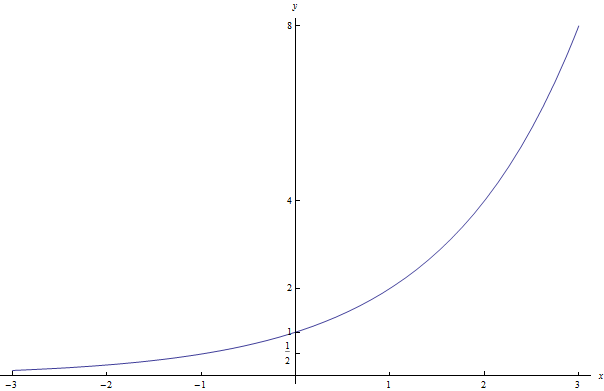
\includegraphics[width=0.6\textwidth]{imagens/2ax_2.png}
	\caption{Gráfico de $f^{-1}(x)=2^x$}
	\label{fig:2ax}
\end{figure}

\textbf{2º Passo: Trace a reta $y=x$ e faça o gráfico de $f(x)$ por reflexão}
\newpage
\margem{ Se fossemos seguir os passos 1 e 2 para traçar o gráfico da função logarítmica de base entre $0$ e $1$, no final teríamos esse esboço: 	
  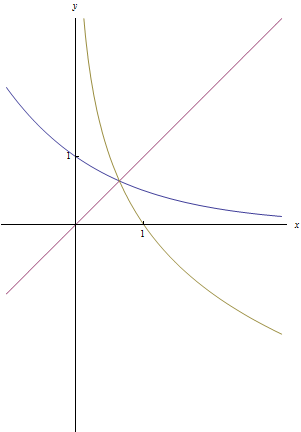
\includegraphics[width=0.85\marginparwidth]{imagens/expneglogneg.png}
	\captionof{figure}{Esboço de $f(x)=log_{\frac{1}{2}}x$ em amarelo e $f^{-1}(x)=\frapar{1}{2}^x$ em azul}
	\label{fig:expneglogneg}
	
	A imagem fica um pouco confusa porque, nesse caso, as curvas se interceptam. Mas note que a reta $y=x$ (em roxo) funciona como um espelho entre os gráficos das duas funções.
	}
\begin{figure}[h]
	\centering
		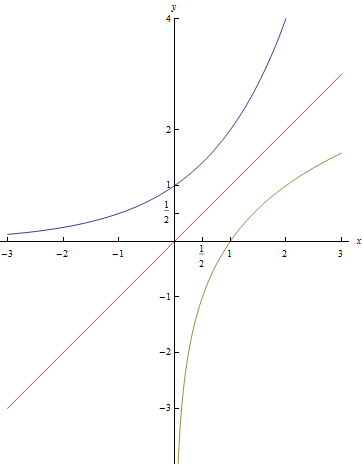
\includegraphics[width=0.6\textwidth]{imagens/2axlog2.png}
	\caption{Gráfico de $f(x)$ e $f^{-1}(x)$, simétricos a reta $y=x$}
	\label{fig:2axlog2}
\end{figure}
De forma semelhante, o gráfico de uma função logaritmica de base $b$ qualquer

\end{document}